\documentclass{article}
\usepackage{amsmath,amsthm}
\usepackage{amssymb,latexsym}
\usepackage{float}
\usepackage{fullpage}
\usepackage{times}

% graphs
\usepackage{tikz}
\usetikzlibrary{automata,positioning}

\tikzset{initial text={}}

\newtheorem{theorem}{Theorem}
\newtheorem{corollary}[theorem]{Corollary}
\newtheorem{question}[theorem]{Question}
\newtheorem{lemma}[theorem]{Lemma}
\newtheorem{observation}[theorem]{Observation}
\newtheorem{proposition}{Proposition}
\newtheorem{definition}[theorem]{Definition}
\newtheorem{claim}[theorem]{Claim}
\newtheorem{fact}[theorem]{Fact}
\newtheorem{assumption}[theorem]{Assumption}
\newtheorem{example}{Example}
\newtheorem{conjecture}[theorem]{Conjecture}
\newtheorem{alg}[theorem]{Algorithm}

\newcommand{\set}[1]{{\left\{#1\right\}}}    % braces for set notation
\newcommand{\ve}[1]{\mathbf{#1}}
\newcommand{\abs}[1]{\left\lvert #1 \right\rvert}
\newcommand{\poly}{\operatorname{poly}}
\newcommand{\complex}{{\mathbb C}}
\newcommand{\reals}{{\mathbb R}}
\newcommand{\ints}{{\mathbb Z}}
\newcommand{\nats}{{\mathbb N}}
\newcommand{\proj}[1]{\mbox{$|#1\rangle \!\langle #1 |$}}
\newcommand{\enc}[1]{\left<#1\right>}
\newcommand{\spa}[1]{\mathcal{#1}}
\newcommand{\ayes}{A_{\rm yes}}
\newcommand{\ano}{A_{\rm no}}

\begin{document}

\title{
    CMSC 303 Introduction to Theory of Computation, VCU\\
    Assignment: 2\\
    Name: Steven Hernandez
}

\date{}

\maketitle
\vspace{-10mm}

\begin{enumerate}
    \item % 1
        \begin{enumerate}
            \item
                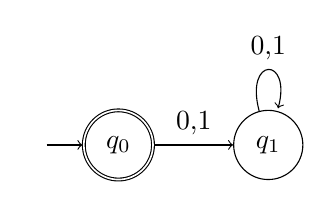
\begin{tikzpicture}
                   \node[state,initial,accepting] (q_0)   {$q_0$};
                   \node[state] (q_1) [right=of q_0] {$q_1$};
                    \path[->]
                    (q_0) edge [above] node {0,1} (q_1)
                    (q_1) edge [loop above] node {0,1} (q_1);
                \end{tikzpicture}
                \\
            \item
                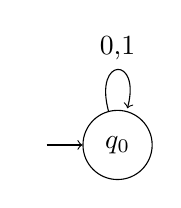
\begin{tikzpicture}
                   \node[state,initial] (q_0)   {$q_0$};
                    \path[->]
                    (q_0) edge [loop above] node {0,1} (q_0);
                \end{tikzpicture}
                \\
            \item
                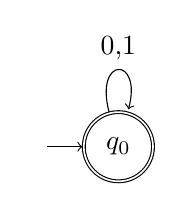
\begin{tikzpicture}
                   \node[state,initial,accepting] (q_0)   {$q_0$};
                    \path[->]
                    (q_0) edge [loop above] node {0,1} (q_0);
                \end{tikzpicture}
        \end{enumerate}
    \item % 2
        \begin{enumerate}
            \item
                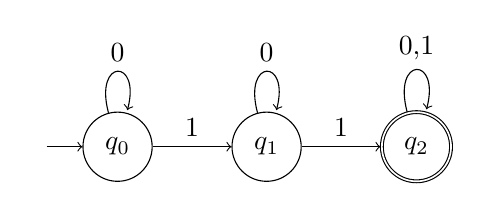
\begin{tikzpicture}
                   \node[state,initial] (q_0)   {$q_0$};
                   \node[state] (q_1) [right=of q_0] {$q_1$};
                   \node[state,accepting] (q_2) [right=of q_1] {$q_2$};
                    \path[->]
                    (q_0) edge [loop above] node {0} (q_0)
                          edge [above] node {1} (q_1)
                    (q_1) edge [loop above] node {0} (q_1)
                          edge [above] node {1} (q_2)
                    (q_2) edge [loop above] node {0,1} (q_2);
                \end{tikzpicture}
                \\
            \item
                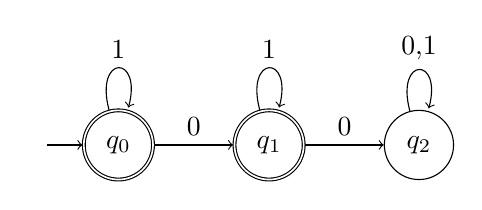
\begin{tikzpicture}
                   \node[state,initial,accepting] (q_0)   {$q_0$};
                   \node[state,accepting] (q_1) [right=of q_0] {$q_1$};
                   \node[state] (q_2) [right=of q_1] {$q_2$};
                    \path[->]
                    (q_0) edge [above] node {0} (q_1)
                          edge [loop above] node {1} (q_0)
                    (q_1) edge [above] node {0} (q_2)
                          edge [loop above] node {1} (q_1)
                    (q_2) edge [loop above] node {0,1} (q_2);
                \end{tikzpicture}
                \\
            \item
                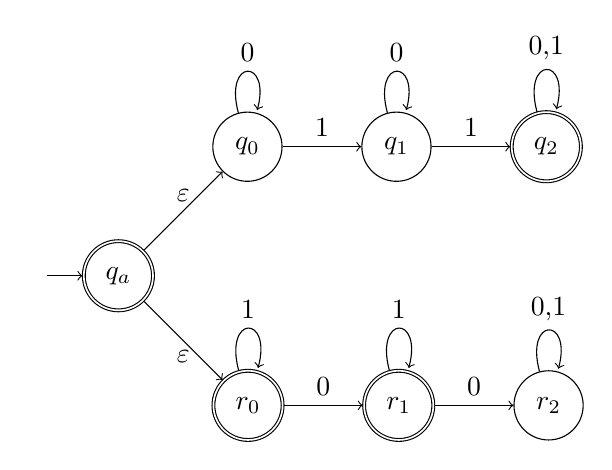
\begin{tikzpicture}
                   \node[state,initial,accepting] (q_a)   {$q_a$};
                   \node[state] (q_0) [above right=of q_a] {$q_0$};
                   \node[state] (q_1) [right=of q_0] {$q_1$};
                   \node[state,accepting] (q_2) [right=of q_1] {$q_2$};
                   \node[state,accepting] (r_0) [below right=of q_a]  {$r_0$};
                   \node[state,accepting] (r_1) [right=of r_0] {$r_1$};
                   \node[state] (r_2) [right=of r_1] {$r_2$};
                    \path[->]
                    (q_a) edge [above] node {$\varepsilon$} (q_0)
                          edge [below] node {$\varepsilon$} (r_0)
                    (q_0) edge [loop above] node {0} (q_0)
                          edge [above] node {1} (q_1)
                    (q_1) edge [loop above] node {0} (q_1)
                          edge [above] node {1} (q_2)
                    (q_2) edge [loop above] node {0,1} (r_2)
                    (r_0) edge [above] node {0} (r_1)
                          edge [loop above] node {1} (r_0)
                    (r_1) edge [above] node {0} (r_2)
                          edge [loop above] node {1} (q_1)
                    (r_2) edge [loop above] node {0,1} (r_2);
                \end{tikzpicture}
        \end{enumerate}
    \item % 3
        This implies regular languages are closed under negation.
        If a DFA $M$ can be designed to recognize B, then applying negation you would have to switch accept and nonaccept states.
        Because the original DFA $M$ was already determined to be have a finite number of steps, then $\bar{B}$ will have the exact same number of steps, thus $\bar{B}$ is also finite and regular.
    \item % 4
        Proof: Let $M_1$ recognize $A$, where $M_1 = (Q_1, \Sigma, \delta_1, q_1, F_1)$, and \\
        $M_2$ recognize $B$, where $M_2 = (Q_2, \Sigma, \delta_2, q_2, F_2)$.

        Construct $M$ to recognize $A \cdot B := \{x | x \in A$ and $x$ does not contain any string in $B$ as a substring.$\}$ where $M = (Q, \Sigma, \delta, q_0, F)$.

        \begin{enumerate}
            \item
                $Q = {(r_1,r_2)|r_1 \in Q_1 and r_2 \in Q_2} \bigcup {\emptyset}$. % TODO: should be null set /0
            \item
                Define $\delta$ such that for $R \in Q$ and any $a \in \Sigma$.

                \[ \delta(R,a) = \begin{cases}
                      \emptyset                                 & R \in F_2     \\%& \set{x | x \in F_2 and x \in R}     & Meaning if any of the states we are on are within F_2, we move directly to \emptyset because the second language was found as a substring of the string, thus this new word cannot be in the new language.
                      \delta(q_1,a) \bigcup \delta(q_2,a)       & R \not\in F_2
                   \end{cases}
                \]
            \item
                $q_0 = (q_1,q_2)$.
            \item
                $F = \set{(r_1,r_2) | r_1 \in F_1$ and $r_2 \not\in F_2}$.
        \end{enumerate}


    \item % 5
        $M$ \\
        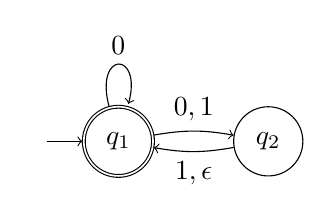
\begin{tikzpicture}
           \node[state,initial,accepting] (q_1)   {$q_1$};
           \node[state] (q_2) [right=of q_1] {$q_2$};
            \path[->]
            (q_1) edge [loop above] node {$0$} (q_1)
                  edge [bend left=10, above] node {$0,1$} (q_2)
            (q_2) edge [bend left=10, below] node {$1,\epsilon$} (q_1);
        \end{tikzpicture}

        $M'$ \\
        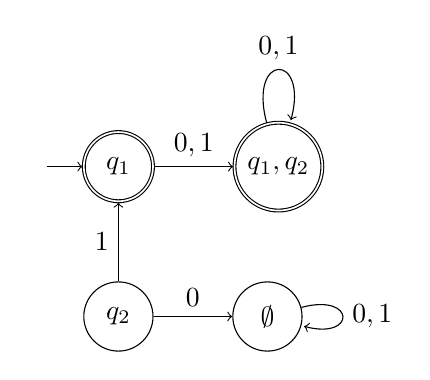
\begin{tikzpicture}
           \node[state,initial,accepting] (q_1)   {$q_1$};
           \node[state,accepting] (q_1q_2) [right=of q_1] {$q_1,q_2$};
           \node[state] (q_2) [below=of q_1] {$q_2$};
           \node[state] (emptyset) [right=of q_2] {$\emptyset$};
            \path[->]
            (q_1) edge [above] node {$0,1$} (q_1q_2)
            (q_1q_2) edge [loop above] node {$0,1$} (q_2)
            (q_2) edge [left] node {$1$} (q_1)
                  edge [above] node {$0$} (emptyset)
            (emptyset) edge [loop right] node {$0,1$} (emptyset);
        \end{tikzpicture}
    \item % 6
        Claim: For any $k, C_k = \Sigma*0\Sigma^{k-1}$ for $k \geq 1$ cannot be recognized by a DFA with less than $2^k$ states.

        Proof: We will begin by taking note of the construction of an NFA for the language $C_k$.
        Notice there must first be a state $q_0$ with transitions: $\delta(q_0, 0) = \set{q_0, q_1} and \delta(q_0, 1) = \set{q_0}$.
        This handles the beginning $\Sigma*0$.

        From $q_1$ must have $k$ additional states to handle counting exactly $\Sigma^{k-1}$ characters after the $0$.
        Each of these states has a transition $\forall a \in \Sigma$ to the next state except the final state.
        This final state is the accept state which has no transitions outbound.
        This is because if we have any additional input, we want the NFA to disregard this branch.

        The number of transitions required for this NFA would be $2 + (k - 1) = k + 1$.

        From our process of transforming NFAs to DFAs, we know that if an NFA has some integer $x$ states, to create a full diagram of all possible transitions, our NFA must contain each element from the Powerset of $x$.
        We also know the $P(x) = 2^x$.

        Seemingly, this proves the claim because $2^{k+1} \geq 2^k$, however, we must take note about $q_0$ from our NFA.

        No matter the input into the NFA, $q_0$ will always be an option for the NFA.
        Thus, $\set{q_0}$ should not be factored into the powerset above.
        So instead, the number of states required for our DFA is $(2^k) + 1 \geq 2^k$ proving the claim.
\end{enumerate}

\end{document}
